\documentclass[aspectratio=169,12pt]{beamer}
\usetheme{Madrid}
\usecolortheme{dolphin}
\usefonttheme{professionalfonts}
\setbeamertemplate{navigation symbols}{}
\setbeamertemplate{footline}{}

\usepackage[T1]{fontenc}
\usepackage[utf8]{inputenc}
\usepackage{graphicx}
\usepackage{amsmath,amssymb}
\usepackage{hyperref}
\usepackage{siunitx}
\usepackage{physics}
\graphicspath{{figures/}}

\title[Chapter 6]{Chapitre 6: Systèmes à 2 qubits et intrication}
\author{JAMOTTE Maxime, SCHOONEN Cédric}
\institute{Digital Learning Hub}
\date{}

\begin{document}

\begin{frame}
  \titlepage
\end{frame}

% \begin{frame}{Table des matières}
%   \tableofcontents
% \end{frame}

% \section{}

\begin{frame}{Objectifs du chapitre 6}
  \begin{enumerate}[<+->]
    \item Représentation tensorielle d'un état à 2 qubits.
    \\~\\
    \item Etats-produits vs intriqués (+exemples)
    \\~\\
    \item Portes quantiques sur 2 qubits
    \\~\\
    \item Générer une paire de Bell
    \\~\\
    \item Conséquences de l'intrication sur la mesure
  \end{enumerate}
\end{frame}

\section{États à deux qubits}

\begin{frame}{1) Représentation tensorielle d'un état à 2 qubits}
  \begin{itemize}[<+->]
    \item État général $\ket{\Psi_2} = a_{00}\ket{00}+a_{01}\ket{01}+a_{10}\ket{10}+a_{11}\ket{11}$ (vecteur de taille $2^2$).
    \\~\\
    \item Produit tensoriel de kets: $\ket{0}_2\!\otimes\!\ket{0}_1=\ket{00}$.
    \\~\\
    \item Nombre d'états de base pour $N$ qubits: $2^N$ (ex.: 2 qubits $\rightarrow$ 4 composantes).
  \end{itemize}
\end{frame}

\begin{frame}{1) Représentation tensorielle d'un état à 2 qubits}
  \begin{itemize}
    \item État général $\ket{\Psi_2} = a_{00}\ket{00}+a_{01}\ket{01}+a_{10}\ket{10}+a_{11}\ket{11}$ (vecteur de taille $2^2$).
    \\~\\
    \item Produit tensoriel de kets: $\ket{0}_2\!\otimes\!\ket{0}_1=\ket{00}$.
    \\~\\
    \item Nombre d'états de base pour $N$ qubits: $2^N$ (ex.: 2 qubits $\rightarrow$ 4 composantes).
  \end{itemize}
  ~\\~\\
  $\qquad \qquad\begin{pmatrix} 
    a_{00}^{} \\
    a_{01}^{} \\
    a_{10}^{}\\
    a_{11}^{} \\
\end{pmatrix} \longrightarrow \ket{00} = \begin{pmatrix} 
    1\\
    0\\
    0\\
    0\\
\end{pmatrix} , \ket{01} = \begin{pmatrix} 
    0\\
    1\\
    0\\
    0\\
\end{pmatrix}, \ket{10} = \begin{pmatrix} 
    0\\
    0\\
    1\\
    0\\
\end{pmatrix} , \ket{11} = \begin{pmatrix} 
    0\\
    0\\
    0\\
    1\\
\end{pmatrix}  $
\end{frame}

\begin{frame}{2) États-produits vs intriqués}
  \begin{itemize}[<+->]
    \item \textbf{État produit}: $\ket{\Psi_2}=\ket{\phi_2}\!\otimes\!\ket{\psi_1}$; évolution \textbf{indépendante} des qubits dans le circuit. Etat produit = état séparable.
    \\~\\
    \item \textbf{Non séparable} = intriqué: mesurer un qubit influence l'autre.
    \\~\\
    \item Paires de Bell: $\ket{\Phi_{\pm}}=\frac{\ket{00}\pm\ket{11}}{\sqrt{2}}$, $\ket{\Psi_{\pm}}=\frac{1}{\sqrt{2}}(\ket{01}\pm\ket{10})$.
    \\~\\
    \item L'état $\ket{00} + \ket{01}$ est-il intriqué? Peut-on le récrire comme un état produit? 
  \end{itemize}
\end{frame}

\begin{frame}{2) Tester l'intrication (décomposition de Schmidt)}
  \begin{itemize}[<+->]
    \item \textbf{Décomposition SVD} $\rightarrow$ coefficients de Schmidt.
    \\~\\
    \item Rang de Schmidt = nombre de coefficients non nuls:\\~\\
    rang 1 $\Rightarrow$ produit, rang $>1$ $\Rightarrow$ intriqué.
    \\~\\
    \item Exemples (notebook): $\frac{\ket{00}+\ket{01}}{\sqrt{2}}$ rang 1; $\ket{\Psi_-}$ rang 2.
  \end{itemize}
\end{frame}

\section{Opérations sur plusieurs qubits}

\begin{frame}{3) Portes quantiques sur deux qubits: portes locales en parallèle}
  \begin{itemize}[<+->]
    \item Action séparée: $(M_2\ket{\psi_2})\!\otimes\!(M_1\ket{\phi_1}) = (M_2\!\otimes\! M_1)(\ket{\psi_2}\!\otimes\!\ket{\phi_1})$.
    \\~\\
    \item Circuit exemple: deux portes de Hadamard appliquées sur deux qubits initiaux $\ket{0}$ et $\ket{1}$.
  \end{itemize}
  \begin{center}
    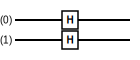
\includegraphics[width=0.3\textwidth]{parallel_hadamard.png}
  \end{center}
\end{frame}

\begin{frame}{3) Portes quantiques à deux qubits: porte SWAP}
  \begin{itemize}[<+->]
    \item Échange les qubits: $\ket{01}\leftrightarrow\ket{10}$ via une matrice $4\times4$ de permutation.
    \\~\\
    \item Ne crée pas d'intrication (seule permutation des composantes).\\~\\
  \end{itemize}
  \[S = \begin{pmatrix}
      1 & 0 & 0 & 0\\
      0 & 0 & 1 & 0\\
      0 & 1 & 0 & 0\\
      0 & 0 & 0 & 1
    \end{pmatrix}
  \]
  \begin{center}
    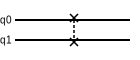
\includegraphics[width=0.3\textwidth]{swap_gate.png}
  \end{center}
\end{frame}

\begin{frame}{3) Portes quantiques à deux qubits: porte CNOT (CX)}
  \begin{itemize}[<+->]
    \item Contrôle sur le deuxième qubit, cible sur le premier.
    \item Retourne la cible si le contrôle vaut $\ket{1}$; matrice $4\times4$ non factorisable $\Rightarrow$ peut intriquer.
  \end{itemize}
  \[
    C_X = \begin{pmatrix}
      1 & 0 & 0 & 0\\
      0 & 1 & 0 & 0\\
      0 & 0 & 0 & 1\\
      0 & 0 & 1 & 0
    \end{pmatrix}
  \]
  \begin{center}
    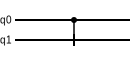
\includegraphics[width=0.3\textwidth]{cnot_gate.png}
  \end{center}
\end{frame}

\begin{frame}{3) Portes quantiques à deux qubits: porte CZ}
  \begin{itemize}[<+->]
    \item Change le signe du coefficient devant $\ket{11}$ seulement.
    \\~\\
    \item Utilisée dans plusieurs algorithmes; peut aussi générer de l'intrication.
  \end{itemize}~\\
  \[
    C_Z = \begin{pmatrix}
      1 & 0 & 0 & 0\\
      0 & 1 & 0 & 0\\
      0 & 0 & 1 & 0\\
      0 & 0 & 0 & -1
    \end{pmatrix}
  \]
  \begin{center}
    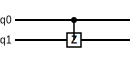
\includegraphics[width=0.32\textwidth]{cz_gate.png}
  \end{center}
\end{frame}

\section{États de Bell}

\begin{frame}{4) Générer une paire de Bell}
  \begin{itemize}[<+->]
    \item Préparation de $\ket{\Phi_+} = (\ket{00}+\ket{11})/\sqrt{2}$: qubits initiaux $\ket{0}$, puis $H$ sur le premier et CNOT.
    \\~\\
    \item Circuit minimal: 2 qubits + 1 porte $H$ + 1 porte CNOT.
  \end{itemize}
  \begin{center}
    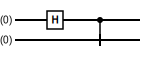
\includegraphics[width=0.4\textwidth]{bell_pair.png}
  \end{center}
\end{frame}

\begin{frame}{5) Conséquences de l'intrication sur la mesure}
  \begin{itemize}
    \item Mesure d'une paire Bell $\ket{\Phi_+}$: résultats corrélés $\ket{00}$ ou $\ket{11}$.
    \item Chaque issue a une probabilité de $0.5$ (environ); \textbf{aucune occurrence} de $01$ ou $10$.
  \end{itemize}
  \begin{center}
    \includegraphics[width=0.45\textwidth]{bell_pair_mesures.png}\hfill
    \includegraphics[width=0.45\textwidth]{bell_hist.png}
  \end{center}
\end{frame}

\begin{frame}{Fin du chapitre 6}
    \centering
  \vfill
  Passons à ...
  \vfill
\end{frame}
\end{document}
